\chapter{Conclusions}
\label{sec:concl}

The way malicious nodes disseminate bogus network information makes the attack resemble fake bootstrapping. In particular, the adversary exploits \texttt{addr} messages exchanges and their relay policy to extensively disperse false network information. 

The efficacy of the strategy has been proven high, as with just 10\% of the identities on the network the adversary can fill peer caches with malicious addresses.

Furthermore, the Sybil attack executed on the new overlay network is substantially more powerful, as it makes coverage drop steeply with less malicious nodes involved in the attack.

It is necessary to point out that the new Sybil attack achieves high efficacy despite working with a network far more dense than the one in the results of Serena et al. Their work assessed the importance of an highly connected graphs as a direct countermeasure to Sybil attacks of this kind.

Therefore, the results obtained imply an increased feasibility of the attack, since the adversary needs to control fewer identities to disrupt honest activities. With just the 20\% of the nodes it is possible to make coverage drop below 40\%.\par

Nonetheless, the setting of the attack is ideal and cannot be compared to that of a real network. The positive outcome is influenced by the increased capability to spread network information during the time the graph topology is still forming.

Under no circumstances the real Bitcoin network could undergo such process. For this reason the attack has been carried out on a second scenario where all the malicious nodes are on fresh bootstrap.

The results in Fig.~\ref{fig:ext-cov} show how the attack was utterly ineffective even though the network was still being built at the time the Sybils started to join.
 
Furthermore, also the new behaviiour of Sybils did not work, since the average percentage of attacking neighbours (Fig.~\ref{fig:ex-atk-neigh}) is significantly lower.

Despite that, there is no gap that big in the rate of Sybils in the peer cache (Fig.~\ref{fig:ex-atk-known}) between the two attack scenarios, thus stating the attackers could still disseminate rather well their addresses.

This means that the positive outcome of the attack in the first scenario was influenced by two factors: the presence of Sybils in the DNS lists and the time at which malicious addresses start to be disseminated.

Although the first factor has been surely influential in later stages of the simulation, when the number of attackers increased, it is required to assess the importance of the latter.

The data in Fig.~\ref{fig:beginning} shows the percentage of malicious addresses in peer caches before bootstrapping nodes start to join in the first attack scenario. In the second no Sybils can be in any peer cache, since they have to join the network first.\par

\begin{figure}[h!]
	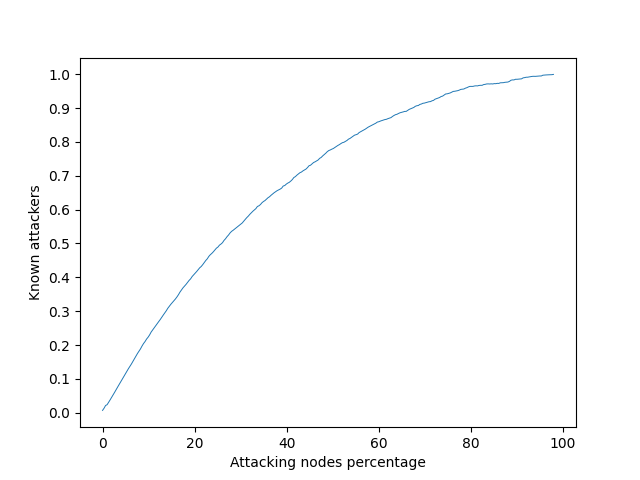
\includegraphics[width=.7\textwidth]{pict/results/in-atkknown-beginning.png}
	\centering
	\caption{Percentage of Sybils in the peer cache at the beginning of the graph construction in the first attack scenario}
	\label{fig:beginning}
\end{figure}

It is evident that honest nodes have a good probability of connecting to a malicious nodes as their first or second neighbour.

Whenever this happens their caches are filled with malicious addresses. From that point on the chance of connecting to another malicious address will be extremely high.

For this reason, the sooner a node connects to a malicious address the more likely it is that it will be eclipsed or have an high amount of Sybils amongst its neighbours.

This cannot happen in the second scenario. Most of the honest nodes have already at least one honest peer at the time malicious nodes start to join. Therefore it is likely that a their second neighbour will be another honest node. Such network is naturally difficult to attack.

Moreover, in this phase \texttt{addr} exchanges between honest nodes cannot contain Sybil addresses.

Lastly, malicious nodes cannot carry out fake bootstrapping, since their addresses are not in DNS lists and as a result bootstrapping honest nodes will surely contact other honest nodes first.

All of these reasons concurrently hinder the success of the attack.

...

To conclude, the major factor for the success of the attack was the presence of Sybils in the network before the attack started.

The new behaviour of the sybils changed the way the graph forms.